\begin{frame}{Percepción Remota}
    \begin{block}{¿Qué es la percepción remota?}
        Técnica o conjunto de técnicas que permite medir y registrar la energía
        electromagnética reflejada o emitida por la superficie de la Tierra y 
        relacionar tales mediciones con su naturaleza y distribución.
    \end{block}    

    \begin{figure}
      \begin{center}
        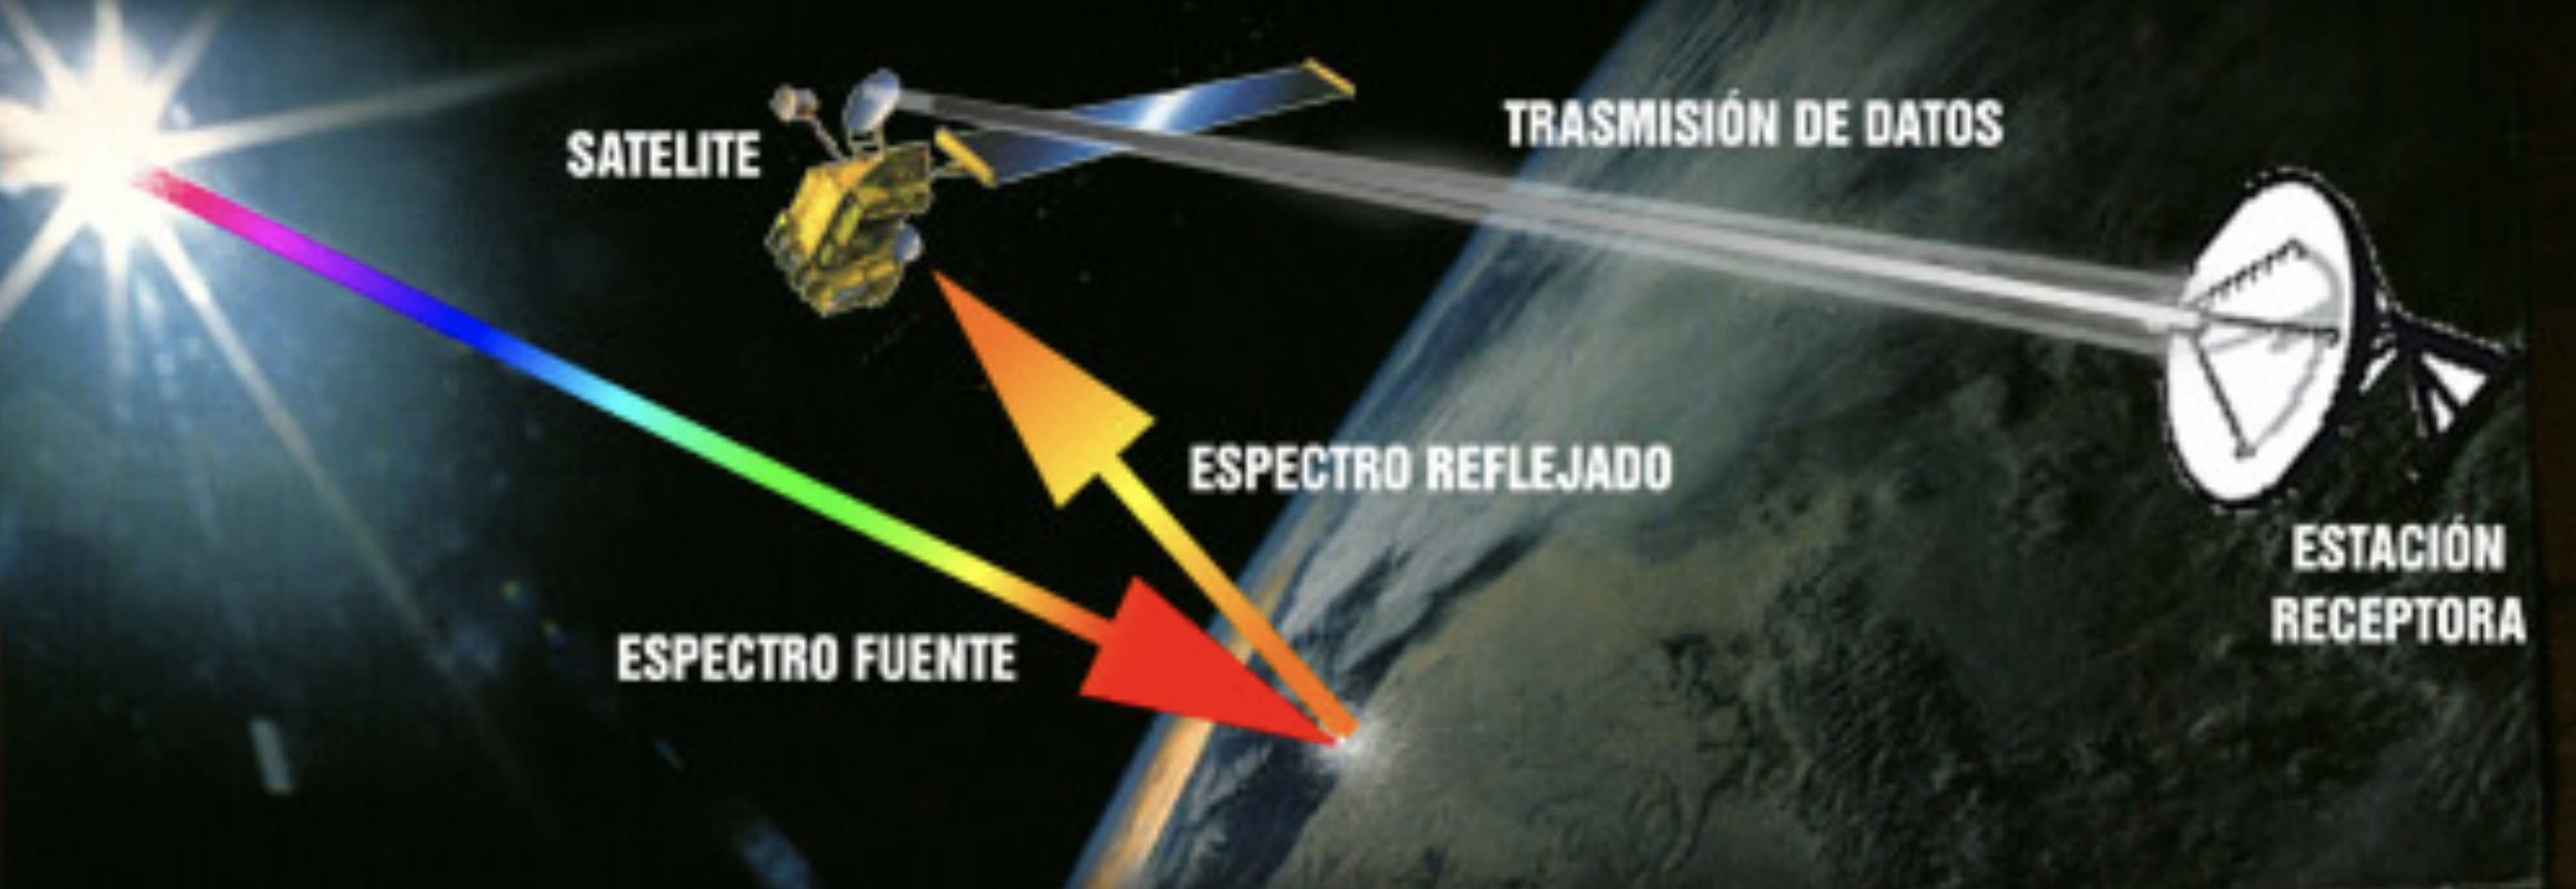
\includegraphics[width=0.95\textwidth]{img/section_03/percepcion_remota}
      \end{center}
      \caption{Fuente: \url{https://haciaelespacio.aem.gob.mx/revistadigital/articul.php?interior=706}}\label{fig:percepcion_remota}
    \end{figure}
    
\end{frame}

\begin{frame}{Sistemas de percepción remota}
  \begin{figure}
    \begin{center}
      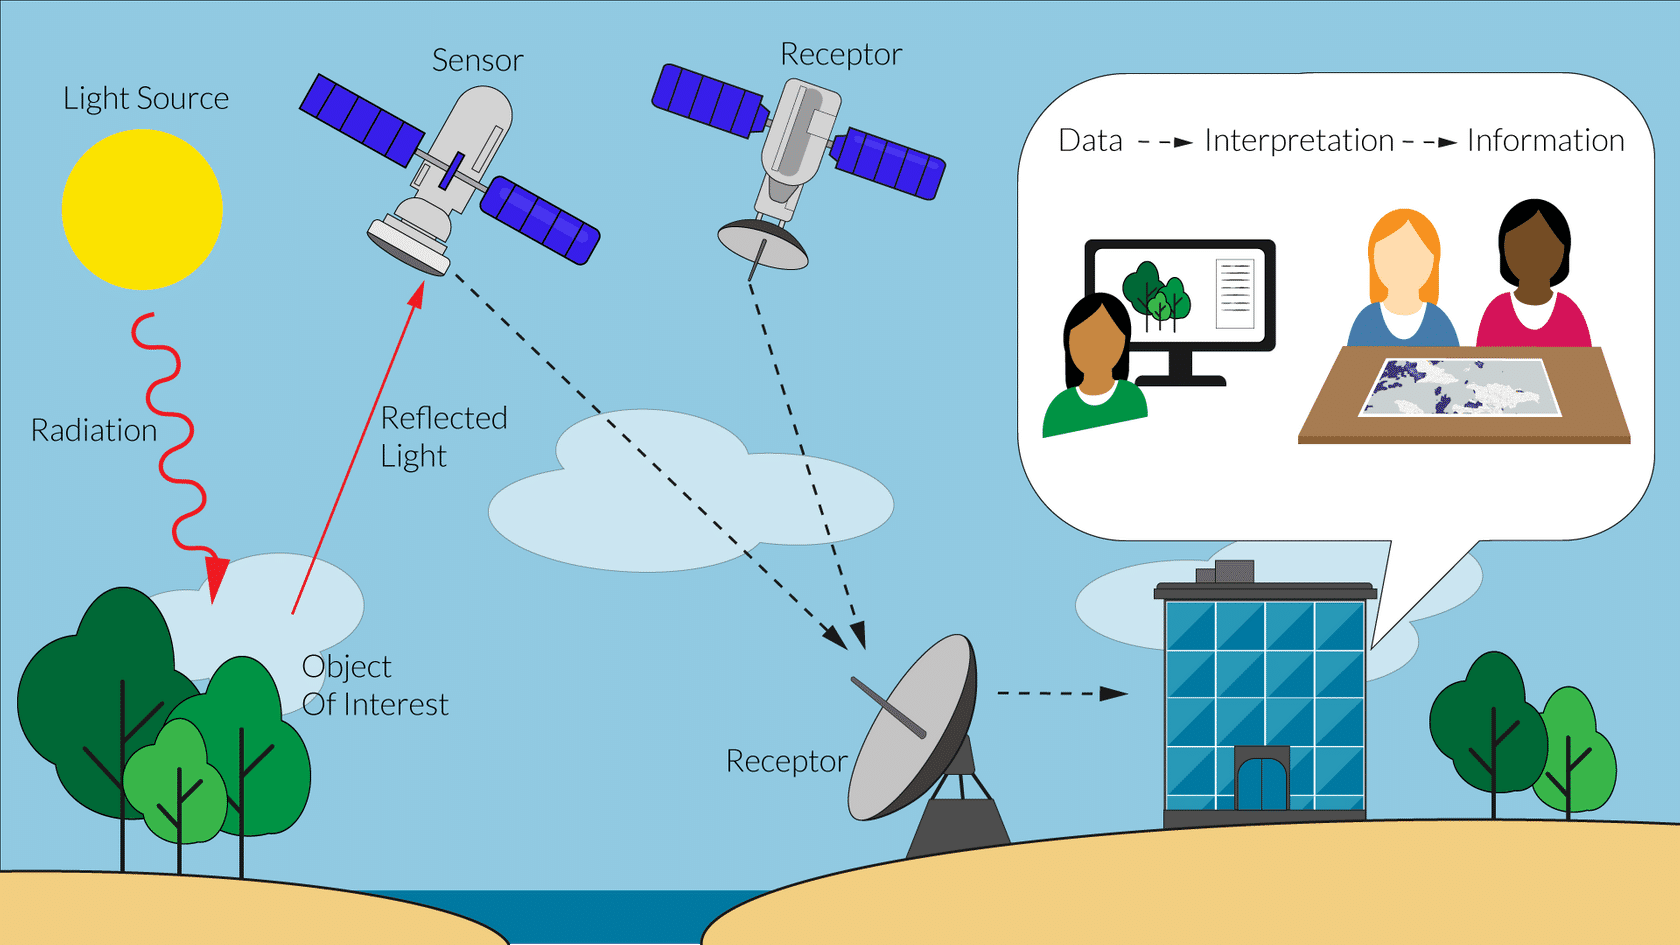
\includegraphics[width=0.95\textwidth]{img/section_03/elementos3.jpg}
    \end{center}
    \caption{Elementos de un sistema de percepción remota}
    \label{fig:elementos_percepcion_remota}
  \end{figure}
\end{frame}
  

\begin{frame}{Tipos de sensores}
    \begin{itemize}
        \item Sensores pasivos.- no poseen una fuente de energía por lo que solo detectan la radiación emitida y/o reflejada por la superficie terrestre que proviene de una fuente externa (como el la luz del sol).
        \item Sensores activos.- poseen una fuente propia de energía que les permite emitir su propia radiación la cuál interactúa con la superficie terrestre y al ser reflejada es captada por el sensor.
    \end{itemize}
    
    \begin{figure}
        \centering
        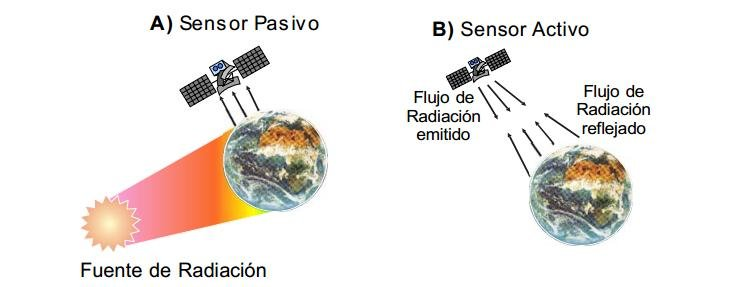
\includegraphics[scale=0.4]{img/section_03/tipos_de_sensores.png}
        \caption{Sensores activos y sensores pasivos \cite{phdthesis}}
        \label{fig:section_03_sensores_activos_pasivos}
    \end{figure}
\end{frame}

\begin{frame}{Espectro eletromagnético}
    \begin{figure}
        \centering
        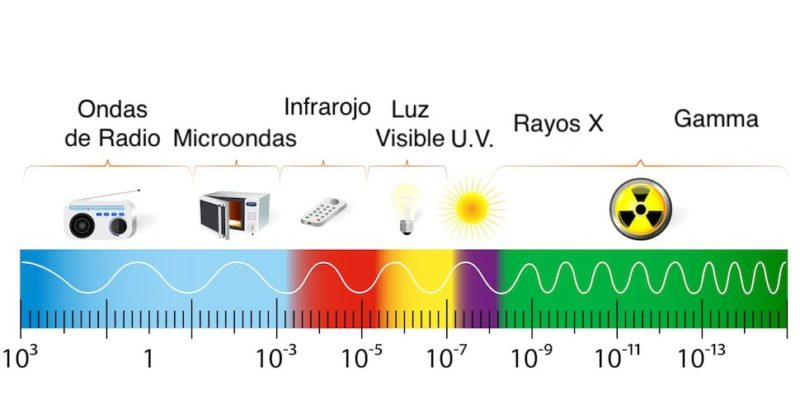
\includegraphics[scale=0.2]{img/section_03/espectro-electromagnetico.jpg}
        \caption{Espectro electromagnético}
        \label{fig:section_03_espectro_electromagnetico}
    \end{figure}
    
    \tiny
    \begin{table}
        \centering
        \begin{tabular}{c|c|c}
            \hline
            Banda & Longitud de onda & Tipo de Instrumentos \\
            \hline
            Radar & 1-30 cm & SLAR/SAR \\
            Microondas & 2-8 mm & Radiómetros \\
            Infrarojo termal & 1-14 um & Videocámaras y escáner de línea \\
            Infrarojo (MIR) & 3-5 um & Videocámaras y escáner de línea \\
            Bajo infrarojo & 1-3 um & Filme y videocámaras \\
            Visual & 350-750 nm & Filme, videocámaras y espectrómetros \\
            Ultravioleta & 250-350 nm & Filme, videocámaras y escáner de línea \\
            \hline
        \end{tabular}
        \caption{Bandas en detección remota}
        \label{tab:bandas_deteccion_remota}
    \end{table}
\end{frame}

\begin{frame}{Resolución}
    
  \begin{block}{Resolución de los sensores remotos}
    La resolución de un sensor es su habilidad para registrar información en detalle de las distintas cubiertas. La resolución depende de la capacidad de los sensores para distinguir variaciones de la energía electromagnética, del detalle espacial que captura y del número y ancho de las bandas que alberga.
  \end{block}
 \end{frame}
    
\begin{frame}{Resolución espacial}
  \begin{block}{Resolución espacial}
    es el objeto más pequeño que puede ser distinguido sobre la imagen. Define el tamaño del píxel, que es la distancia correspondiente al tamaño de la mínima unidad de información en la imagen.
  \end{block}

  \begin{figure}
    \begin{center}
      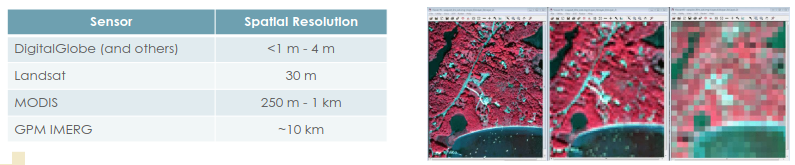
\includegraphics[width=0.95\textwidth]{img/section_03/resolucion_espacial}
    \end{center}
    \caption{Fuente: Fundamentals of Remote Sensing - NASA Applied Sciences}
    \label{fig:resolucion_multiespectral_vs_hiperespectral}
  \end{figure}
\end{frame}

\begin{frame}{Resolución espectral}
  \begin{block}{Resolución espectral}
    es el número y el ancho de las bandas espectrales que puede discriminar el sensor, monoespectrales y multiespectrales. Típicamente un sensor multiespectral tiene de 3 a 10 bandas mientras que uno hiperespectral puede contener cientos de ellas.
  \end{block}

  \begin{figure}
    \begin{center}
      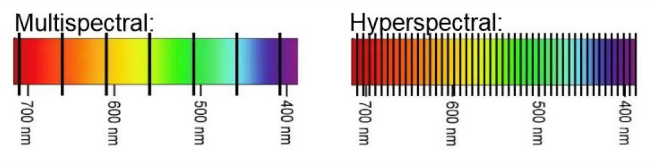
\includegraphics[width=0.95\textwidth]{img/section_03/resolucion_espectral}
    \end{center}
    \caption{Fuente: Fundamentals of Remote Sensing - NASA Applied Sciences}
    \label{fig:resolucion_espectral}
  \end{figure}
  
\end{frame}

\begin{frame}{Resolución radiométrica}
  \begin{block}{Resolución radiométrica}
    es la capacidad para detectar variaciones en la radiancia espectral que recibe. Determina el número de niveles de gris recogidos y se expresa en niveles por píxel. A mayor resolución radiométrica, mejor interpretación de la imagen.
  \end{block}

  \begin{figure}
    \begin{center}
      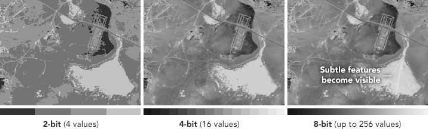
\includegraphics[width=0.80\textwidth]{img/section_03/resolucion_radiometrica}
    \end{center}
    \caption{Fuente: Fundamentals of Remote Sensing - NASA Applied Sciences}
    \label{fig:resolucion_radiometrica}
  \end{figure}
\end{frame}

\begin{frame}{Resolución temporal}
  \begin{block}{Resolución temporal}
    es la periodicidad con que el sensor adquiere imágenes de la misma porción de la superficie terrestre. Esta en función de las características orbitales de la plataforma (altura, velocidad e inclinación) y del diseño del sensor (ángulo de observación y ángulo de cobertura).
  \end{block}

  \begin{figure}
    \begin{center}
      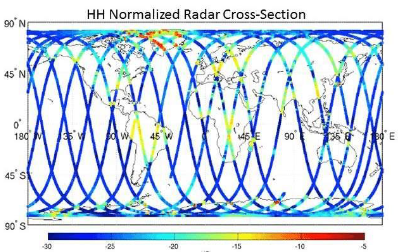
\includegraphics[scale=0.4]{img/section_03/resolucion_temporal}
    \end{center}
    \caption{Fuente: Fundamentals of Remote Sensing - NASA Applied Sciences}
    \label{fig:resolucion_temporal}
  \end{figure}
\end{frame}

\begin{frame}{Radar de Apertura Sintética}
    \footnotesize
    
    \begin{itemize}
        \item Sensor activo.- emite microondas ($f_0 = 1-30 Ghz$) con cierto ángulo de incidencia ($\theta_i = 20-65°$) y forma imágenes con el eco $\sigma^0$ de la radiación emitida.

        \item Apertura sintética.- integra la historia de $\sigma^0$ durante un cierto tiempo $T_i$ a lo largo de la trayectoria de vuelo del sensor y con ello \textit{sintetiza} una antena $L_{SAR} >> L_{real}$

        \item Formación de la imagen.- basada en el principio de retrodispersión de las microondas por parte de las ondas de Bragg.
    \end{itemize}

    \begin{figure}
        \centering
        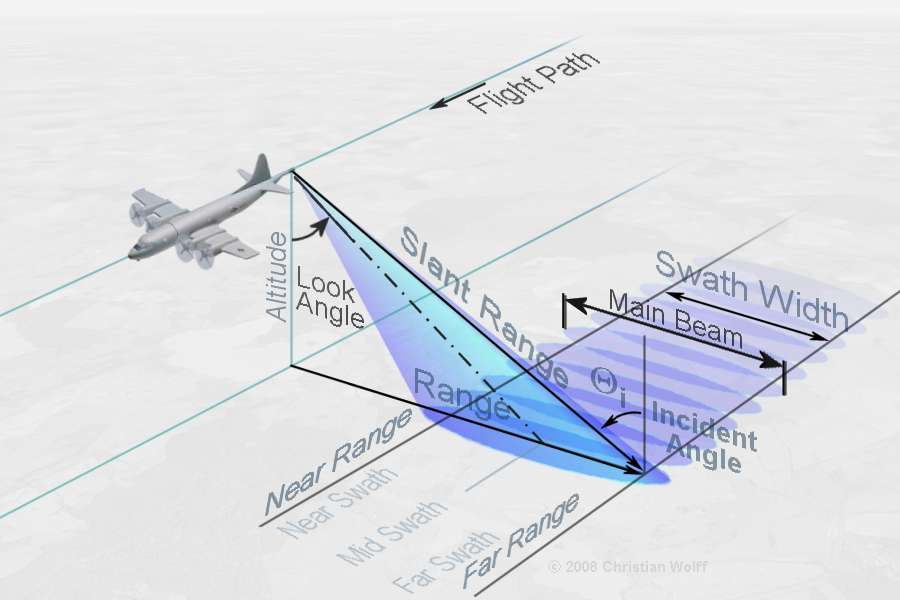
\includegraphics[scale=0.2]{img/section_03/SLAR-geometry_p.jpg}
        \caption{Radar de apertura sintética}
        \label{fig:section_03_radar_apertura_sintetica}
    \end{figure}
\end{frame}

\begin{frame}{Principios de formación de la imagen de radar}
  \begin{block}{Fundamento básico}
    El fundamento básico de una imagen de radar es un sensor que emite un pulso y a través de la diferencia en el transcurso de tiempo entre su emisión y recepción así como de la amplitud del pulso retornado, se puede obtener la distancia del sensor a la que se encuentra el objeto en el que rebotó el pulso.
  \end{block}

  \begin{figure}
    \begin{center}
      \begin{tabular}[c]{ll}
        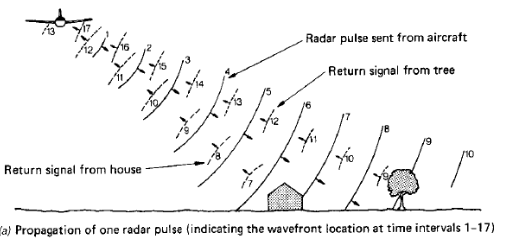
\includegraphics[scale=0.3]{img/section_03/principio_01} &
        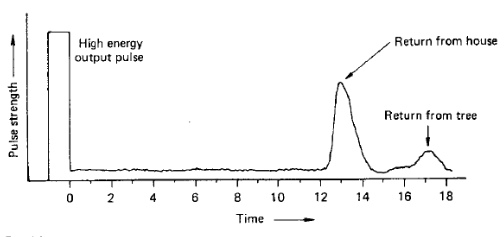
\includegraphics[scale=0.3]{img/section_03/principio_02} \\
      \end{tabular}
    \end{center}
    \caption{Fuente: Fundamentos de teledetección radar. Gobierno de España}
    \label{fig:resolucion_temporal}
  \end{figure}
\end{frame}

\begin{frame}{Frecuencias de operación}
  \begin{block}{Frecuencias}
    Los radares trabajan en la frecuencia del espectro electromagnético de las microondas (por lo que también son llamados sensores de microondas) pero se subdividen en los siguientes grupos
  \end{block}

  \footnotesize
  \begin{table}
    \caption{Longitudes de onda y frecuencias de radar}
    \label{tab:longitudes_onda}
    \begin{center}
      \begin{tabular}[c]{c|l|l}
        \hline
        Banda & Longitud de onda (cm) & Frecuencia (GHz) \\
        \hline
        Ka & 0.75 - 1.2 & 40 - 25 \\
        K & 1.2 - 1.67 & 25 - 18 \\
        Ku & 1.7 - 2.5 & 17.6 - 12 \\
        X & 2.5 - 4 & 12 - 7.5 \\
        C & 4 - 8 & 7.5 - 3.75 \\
        S & 8 - 15 & 3.75 - 2 \\
        L & 15 - 30 & 2 - 1 \\
        P & 60 - 120 & 0.5 - 0.25 \\
        \hline
      \end{tabular}
    \end{center}
  \end{table}
\end{frame}

\begin{frame}{Apertura sintética}
  \begin{block}{Antena de apertura sintética}
    Existe una relación proporcional entre la ganacia observada sobre la retrodispersión y la longitud de la antena de un radar, esto implica que para obtener una resolución radiométrica suficiente para poder distinguir las escalas de operación requeriríamos de antenas físicas muy largas lo cuál complica su procedimiento de instalación y operación
  \end{block}

  \begin{figure}
    \begin{center}
        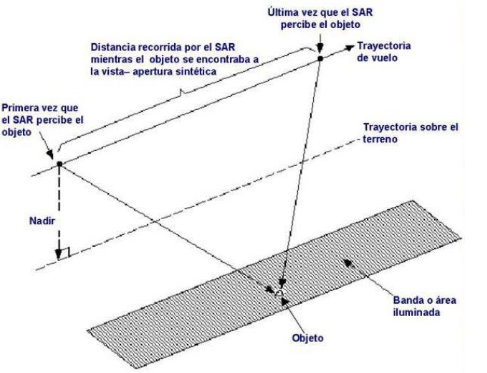
\includegraphics[scale=0.3]{img/section_03/principio_03}  \\
    \end{center}
    \caption{Fuente: Fundamentos de teledetección radar. Gobierno de España}
    \label{fig:resolucion_temporal}
  \end{figure}
\end{frame}

\begin{frame}{Efectos y distorsiones geométricas}
  \footnotesize
  \begin{block}{Efectos}
    Debido al ángulo de inclinación en que la señal se envía y regresa las imágenes de radar sufren de distorsiones debido a efectos geométricos causados por la interacción entre el pulso de radar y la superficie observada
    \tiny
    \begin{itemize}
      \item Escorzo (foreshortening).- compresión de partes de la escena
      \item Inversión por relieve (layover).- diferencias en el tiempo de recepción de la energía reflejada
      \item Sombas (shadow).- zonas no iluminadas por el sensor
    \end{itemize}
  \end{block}

  \begin{figure}
    \begin{center}
        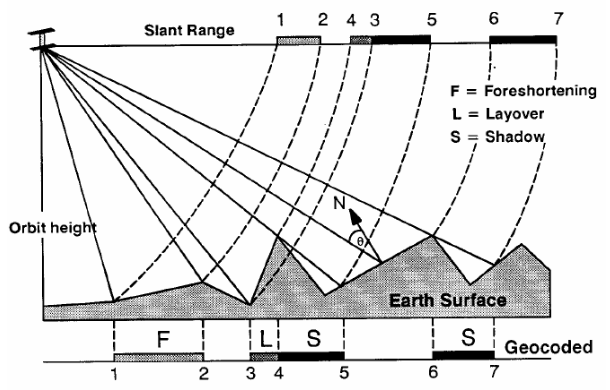
\includegraphics[scale=0.3]{img/section_03/principio_04}  \\
    \end{center}
    \caption{Fuente: Fundamentos de teledetección radar. Gobierno de España}
    \label{fig:resolucion_temporal}
  \end{figure}
\end{frame}
  
\begin{frame}{Retrodispersión}
  \footnotesize
  \begin{block}{Coeficiente de retro-dispersión}
    A diferencia de la percepción óptica las longitudes de onda en detección por radar son lo suficientemente grandes como para poder penetrar cierto tipo de superficies, de forma que la dipersión será el resultado de la combinación de la dispersión producida por la superficie (forma del objeto y propiedades dieléctricas), por su interior e incluso por capas de material mas profundo
  \end{block}

  \begin{figure}
    \begin{center}
      \begin{tabular}[c]{ll}
        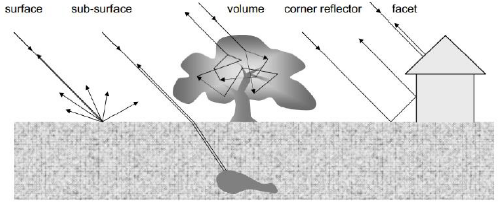
\includegraphics[scale=0.3]{img/section_03/principio_05} &
        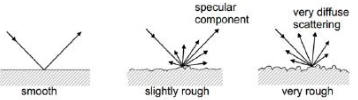
\includegraphics[scale=0.4]{img/section_03/principio_06} \\
      \end{tabular}
    \end{center}
    \caption{Fuente: Fundamentos de teledetección radar. Gobierno de España}
    \label{fig:resolucion_temporal}
  \end{figure}
\end{frame}

\begin{frame}{Ejemplos}
  \footnotesize
  \begin{block}{Valores de retrodispersión}
    Debido a las propiedades anteriores, los valores del coeficiente de retro-dispersión ($\sigma$), medido en dB (decibeles) nos permite asociarlo con diferentes tipos de superficie (observados comunmente en las imágenes de radar), aunque recuerden (IMPORTANTE) no estamos observando una imágen óptica (su principio físico es diferente)
  \end{block}

  \tiny
  \begin{table}
    \caption{Valores de retrodispersión y superficies típicas}
    \label{tab:retrodispersion_superficies}
    \begin{center}
      \begin{tabular}[c]{c|l}
        \hline
        Valores de retro-dispersión & Superficies típicas \\
        \hline
        Muy alto (más de -5 dB) & 
        Objetos antropogénicos (ambientes urbanos), Pendientes orientadas hacia el sensor \\
        Alto (de -10 dB a 0 dB) & Superficies rugosas, vegetación densa (bosques) \\
        Moderado (de -20 a -10 dB) & Niveles medios de vegetación, cultivos, superficies moderadamente rugosas. \\
        Bajo (menos de -20 dB) & Superficies lisas, aguas en calma, carreteras, suelos muy secos (arenas). \\
        \hline
      \end{tabular}
    \end{center}
  \end{table}
\end{frame}

\begin{frame}{Ejemplo de una imagen SAR}
    \begin{figure}
        \centering
        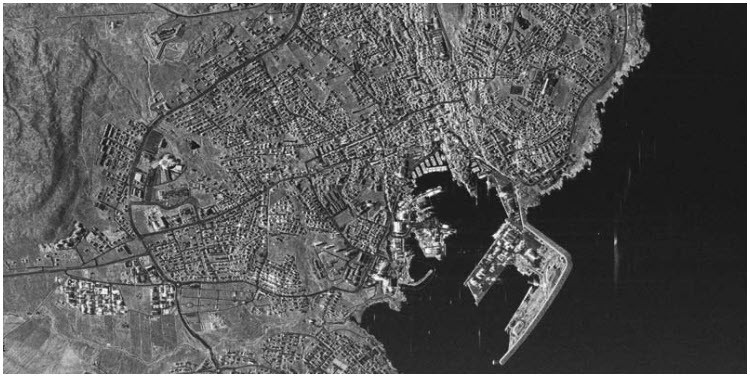
\includegraphics[scale=0.4]{img/section_03/principios_basicos}
        \caption{Fuente: SAR Tutorial, Airbus Defense and Space}
        \label{fig:section_03_dinamica_sar_petroleo}
    \end{figure}
\end{frame}

\begin{frame}{Dinámica de la interacción SAR-Derrame}
  \begin{block}{Cómo detectamos petróleo en el oceano}
    La interacción del pulso del radar en el océano consiste en la dispersión de la señal hacia todas las direcciones por el movimiento de las olas (dispersión de Bragg), el petróleo al ser mas denso, inhibe esta dispersión provocando que la superficie del océano funcione como un espejo (existe baja retrodispersión ya que la señal se refleja).
  \end{block}

    \begin{figure}
        \centering
        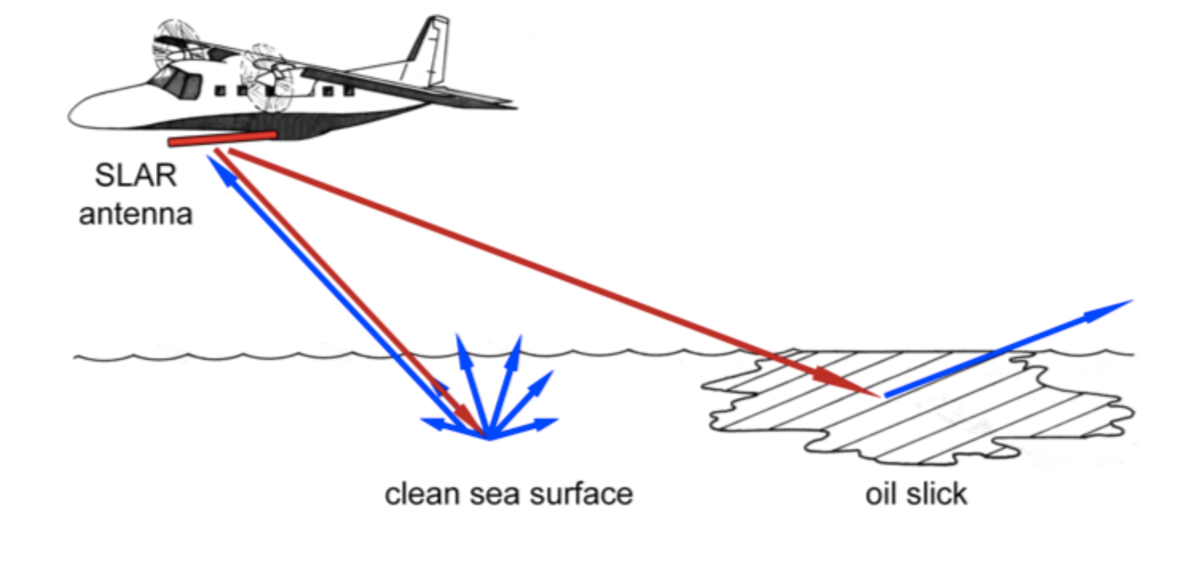
\includegraphics[scale=0.2]{img/section_03/sar-petroleo.png}
        \caption{Dinámica de la interacción entre el pulso del radar y la superficie del derrame de petróleo}
        \label{fig:section_03_dinamica_sar_petroleo}
    \end{figure}
\end{frame}

\begin{frame}{Ejemplo}
    \begin{figure}
        \centering
        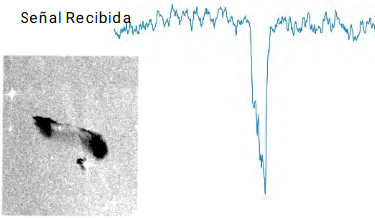
\includegraphics[scale=0.5]{img/section_03/senal_petroleo}
        \caption{Ejemplo de la superficie de un derrame en el océano observada por un sensor de radar}
        \label{fig:section_03_dinamica_sar_petroleo}
    \end{figure}
\end{frame}

\begin{frame}{Ejemplo de una imagen SAR}
    \begin{figure}
        \centering
        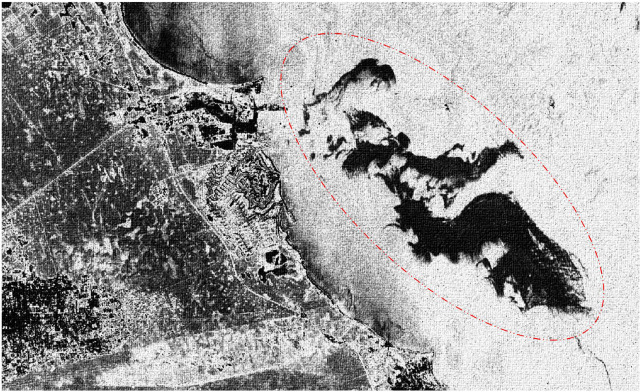
\includegraphics[scale=0.6]{img/section_03/oil_slick}
        \caption{Fuente: SAR Tutorial, Airbus Defense and Space}
        \label{fig:section_03_dinamica_sar_petroleo}
    \end{figure}
\end{frame}

\begin{frame}{Las imágenes no son uniformes}
    \begin{figure}
        \centering
        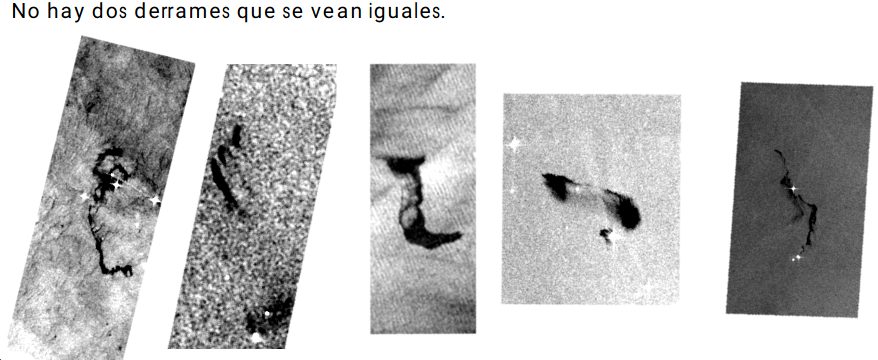
\includegraphics[scale=0.35]{img/section_03/oil_slick_02}
        \caption{Fuente: Malin Johansson, Evaluación de desastres usando Radar de Apertura Sintética}
        \label{fig:section_03_dinamica_sar_petroleo}
    \end{figure}
\end{frame}

\begin{frame}{Otros fenómenos}
    \begin{figure}
        \centering
        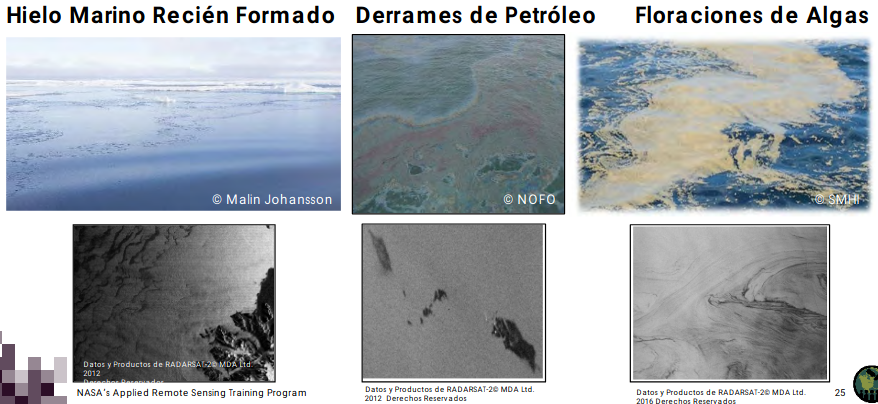
\includegraphics[scale=0.35]{img/section_03/oil_slick_03}
        \caption{Fuente: Malin Johansson, Evaluación de desastres usando Radar de Apertura Sintética}
        \label{fig:section_03_dinamica_sar_petroleo}
    \end{figure}
\end{frame}

